\section{Entangled Qubits and Bell states}

\subsection{Entanglement}


To make two qubits entangled we need to make them dependent on each other, meaning that measuring one of the qubits gives us information about the output of the other. An intuitive approach would be to use a controlled gate, since the effect of the gate on the target qubit changes based on the state of the control qubit.
We start with two qubits in the $\ket{0}$ state.

\begin{equation}
    \begin{array}{cc}
        \textbf{Quantum Circuit:}  & \textbf{State after applied gates:} \\
        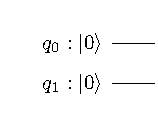
\includegraphics[scale=1.5, valign=c]{Figures/Circuits/Theory/2zero.pdf} &  \ket{q_1 q_2} = \ket{00} \; .
    \end{array}
\end{equation}

Then to put both qubit in a superposition we apply the Hadamard gate to each of them:

\begin{equation}\label{eq:2hadamard}
    \begin{array}{cc}
        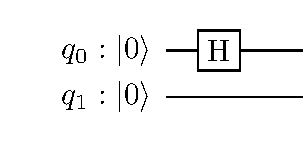
\includegraphics[valign=c]{Figures/Circuits/Theory/2hadamard.pdf} &  \ket{q_1 q_2} = \frac{\sqrt{2}}{2} |00\rangle+\frac{\sqrt{2}}{2} |10\rangle \; .
    \end{array}
\end{equation}


In doing so the first qubit becomes maximally mixed, meaning the first qubit is equally likely to be measured either $\ket{0}$ or $\ket{1}$, as seen in \ref{eq:2hadamard}. Still, the second qubit stays unchanged at $\ket{0}$, so measuring one of the qubits in \ref{eq:2hadamard} would not give us any information about the other. We apply then a \textbf{CNOT} gate:

\begin{equation}\label{eq:Bell1}
    \begin{array}{cc}
        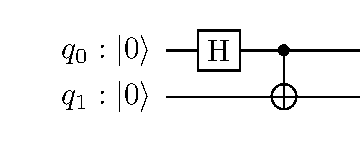
\includegraphics[valign=c]{Figures/Circuits/Theory/HadaCNOT.pdf} &  \ket{q_1 q_2} = \frac{\sqrt{2}}{2} |00\rangle+\frac{\sqrt{2}}{2} |11\rangle \; .
    \end{array}
\end{equation}

The \textbf{CNOT} gate makes it so that measuring $q_0 = \ket{0}$ tells us that $q_1 = \ket{0}$, while measuring $q_0 = \ket{1}$ makes it guaranteed that $q_1 = \ket{1}$, and vice versa. These linked measured values is what constitutes an entanglement of qubits.

\subsection{Bell States}

The resolving entangled state \ref{eq:Bell1} is one of the four maximally entangled states of a two-qubit system called the Bell states. There are four of them because of the four combination of initial states our two-qubit system can be in. We have the first one with initial state $\ket{00}$:

\begin{equation}\label{eq:00Bell}
    \begin{array}{cc}
        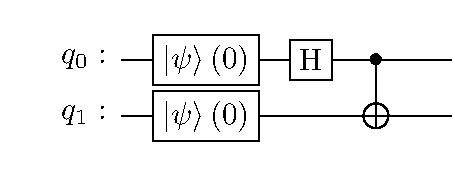
\includegraphics[scale=0.9, valign=c]{Figures/Circuits/Theory/00Bell.pdf} &  \ket{\Phi^+} = \frac{\sqrt{2}}{2} |00\rangle+\frac{\sqrt{2}}{2} |11\rangle \; .
    \end{array}
\end{equation}

For initial state $\ket{10}$:

\begin{equation}\label{eq:10Bell}
    \begin{array}{cc}
        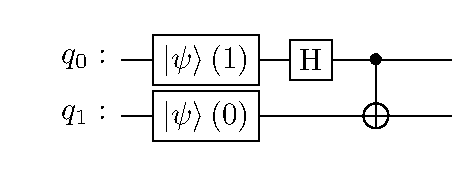
\includegraphics[scale=0.9, valign=c]{Figures/Circuits/Theory/10Bell.pdf} &  \ket{\Phi^-} = \frac{\sqrt{2}}{2} |00\rangle-\frac{\sqrt{2}}{2} |11\rangle \; .
    \end{array}
\end{equation}

And for $\ket{01}$

\begin{equation}\label{eq:01Bell}
    \begin{array}{cc}
        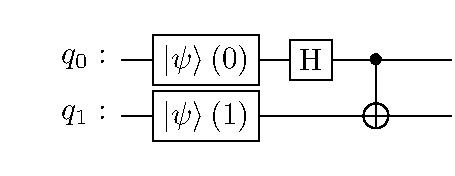
\includegraphics[scale=0.9, valign=c]{Figures/Circuits/Theory/01Bell.pdf} &  \ket{\Psi^+} = \frac{\sqrt{2}}{2} |10\rangle+\frac{\sqrt{2}}{2} |01\rangle \; .
    \end{array}
\end{equation}

And lastly $\ket{11}$:

\begin{equation}\label{eq:11Bell}
    \begin{array}{cc}
        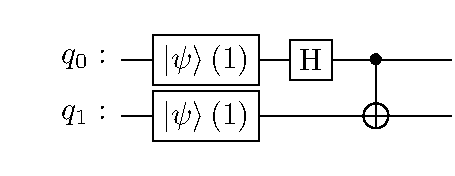
\includegraphics[scale=0.9, valign=c]{Figures/Circuits/Theory/11Bell.pdf} &  \ket{\Psi^-} = \frac{\sqrt{2}}{2} |10\rangle-\frac{\sqrt{2}}{2} |01\rangle \; .
    \end{array}
\end{equation}